\documentclass[tikz, border=0.2cm]{standalone}
\usepackage{tikz}
\begin{document}
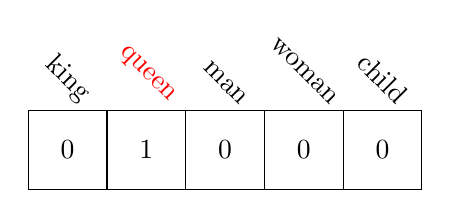
\begin{tikzpicture}
    \draw[step=1cm] (0,0) grid (5,1);
    \node[label={[label distance=2mm]above:\rotatebox{-45}{king}}              ] at (0.5,0.5) {0};
    \node[label={[label distance=2mm]above:\rotatebox{-45}{\color{red}{queen}}}] at (1.5,0.5) {1};
    \node[label={[label distance=2mm]above:\rotatebox{-45}{man}}               ] at (2.5,0.5) {0};
    \node[label={[label distance=2mm]above:\rotatebox{-45}{woman}}             ] at (3.5,0.5) {0};
    \node[label={[label distance=2mm]above:\rotatebox{-45}{child}}             ] at (4.5,0.5) {0};
\end{tikzpicture}
\end{document}
